\documentclass[annual]{acmsiggraph}
\usepackage{wrapfig}
\title{X\textsuperscript{2}-Toon: An Extended X-Toon Shader}

\author{Robert Wolfe\thanks{e-mail:robert\_wolfe@carleton.ca}\\Spencer Elliott\thanks{e-mail:spencer\_elliott@carleton.ca}}
\pdfauthor{Robert Wolfe, Spencer Elliott}

\keywords{xtoon, image processing, xna}

\begin{document}

\maketitle

\begin{abstract}

X-toon ~\cite{BTM06a} extended classic cel shading.

\end{abstract}

\keywordlist

\copyrightspace

\section{Introduction}

We first developed a standard cel shader using ~\cite{CelShadingTut} as a basic example.

We used the GUI framework for XNA from ~\cite{Ruminate}.

\section{Tone Detail}
\begin{wrapfigure}{r}{0.1\textwidth}
  \vspace{-20pt}
  \begin{center}
    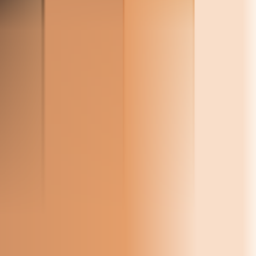
\includegraphics[width=0.1\textwidth]{images/xtoon_skin}
  \end{center}
  \caption{2D Texture.}
  \vspace{-10pt}
  \label{fig:2dtexture}
\end{wrapfigure}
We extend the concept of a regular toon shader by adding a second dimension to the texture. While the x-axis remains as $N\cdot L$, where {\it{N}} is the surface normal and {\it{L}} is the light direction, the y-axis represents the level of detail. The higher up on the axis, the less detail is used. Conversely, the lower the y-axis value, the more detail. An example of a 2D texture used in this application can be seen in Figure~\ref{fig:2dtexture}.

The method of computing the y-axis depends on an {\it{attribute map.}} The chosen attribute changes the level of detail, depending on its value. The original paper provided two possible attribute maps: distance and orientation. This paper deals exclusively with the distance attribute mapping. We provide an alternative mapping involving the angle between the camera {\it{look at}} vector and surface normal. 

In addition to providing an alternate attribute mapping, we also developed a new method for determining the amount of shading on a model. This method involves calculating direction vectors to each light from each vertex. The resulting vector can then be used to calculate the final shading amount.

\subsection{Distance}
We developed a new method to determine the x-axis value based on the lighting of a scene. The direction to each light in the scene is determined for every vertex. These directions would then be summed and a resulting direction vector would be created. The direction vector is normalized and the final detail is calculated using the same equation for determining the 

\subsection{Angle}
We introduce a new attribute map based on the angles of the {\it{look at}} of the camera and the surface normal. The look at vector is the direction that the camera is pointed. The angle between the two vectors is calculated using Equation~\ref{eqn:angle}, which is derived from the formula for dot product.

\begin{equation}
\label{eqn:angle}
a = \cos^{-1}{(-LookAt \cdot Normal / |LookAt||Normal|)}
\end{equation}

\section{Extensions to original X-Toon shader}
We have extended the original shader offered in the X-Toon paper to increase the usability for various new effects. The first extension involves using colours from the original model's textures when calculating the final detail. The second extension allows for the use of transparency in both the tone texture and original model's textures to create 

\subsection{Texture blending}
We have added the ability to blend textures from a model into the calculation of the shading and tone detail. This technique gives artists the ability to retain the original look of the model while also applying the X-Toon effects. To achieve this effect, our shader first takes the pixel sample from the original texture. The shading and detail are determined using the calculations explained in previous sections and the final tone detail pixel is kept. To mix the colours of the original texture and the tone detail pixel, a simple multiplication of the {\it{RGB}} channels is performed. The resulting pixel is a blend of the original texture pixel and the sampled tone detail texture. Figure~\ref{fig:texturing} shows an example of a model with and without texture blending.

\begin{figure}
	\centering
	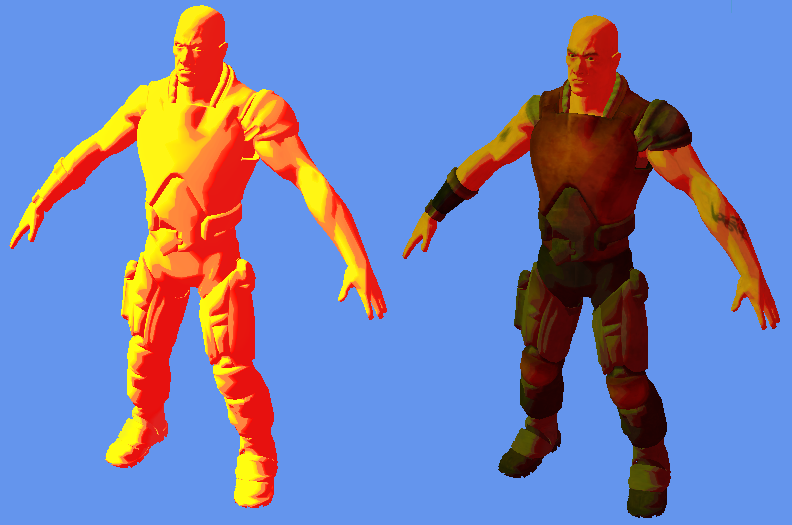
\includegraphics[width=2.5in]{images/textures}
	\caption{A model without and with original textures applied, respectively}
	\label{fig:texturing}
\end{figure}

\subsection{Texture transparency}


\begin{figure}
	\centering
	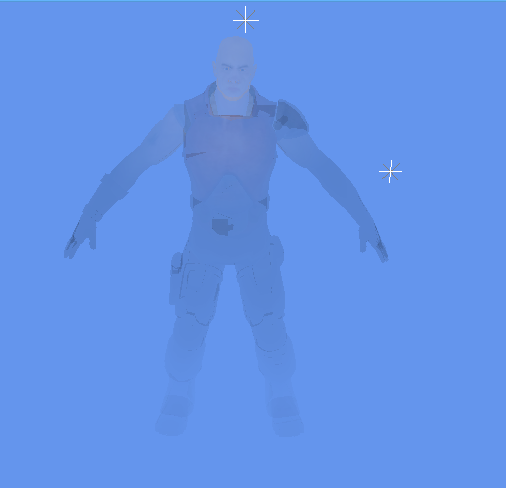
\includegraphics[width=2.5in]{images/transparency}
	\caption{Transparency affecting output}
	\label{fig:transparency}
\end{figure}

\section{Results}

\begin{figure}[ht]
  \centering
  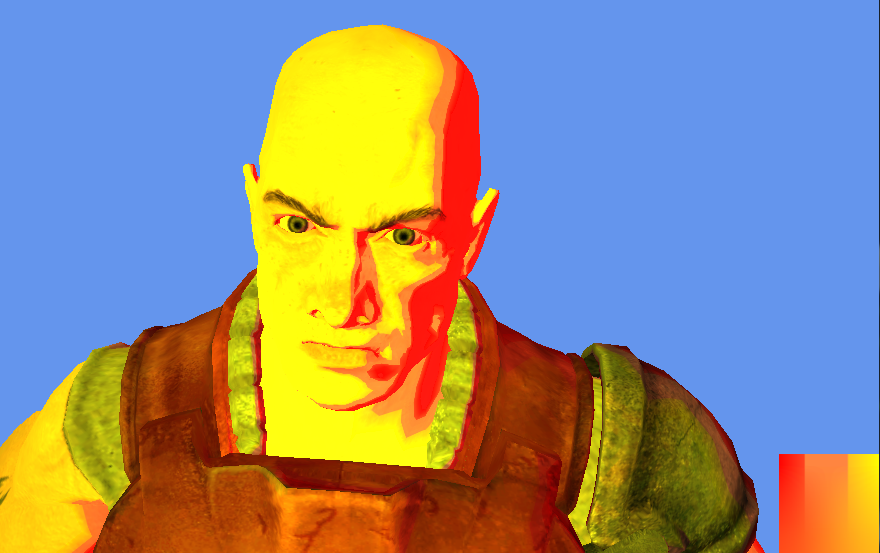
\includegraphics[width=2.5in]{images/test}
  \caption{Sample illustration.}
\end{figure}


\section{Discussion and Future Work}

\subsection{Alpha blending correction}


\section{Conclusion}


\bibliographystyle{acmsiggraph}
\bibliography{paper}
\end{document}
